\newpage
\chapter{Изработване на електронна игра}
\label{chapter02}

\section{Избор на развойни средства}

История на мобилните устройства.

Symbinan, Blackberry, PocketPC

История на iOS.

Objective-C, Swift

История на Android.

Java, Kotlin

\subsection{Избор на развойни инструменти}

\section{Стратегии за проектиране}

\subsection{Трислоен софтуерен модел}

Съвременните тенденции за разработка на софтуер често залагат на многослойни архитектурни решения. Един от най-популярните модели е с три слоя (Фиг. \ref{figure03}). Деленето на трите слоя обхващат визуализацията, обектно-ориентираният модел на данните и съхранението в енергонезависима памет (релационен модел). 

\begin{figure}[h!]
 \centering
 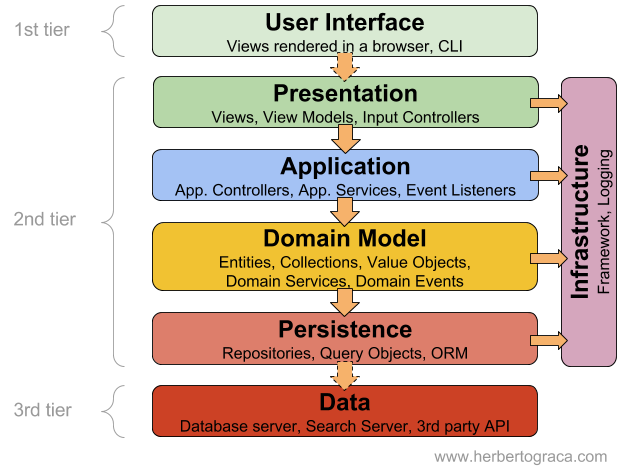
\includegraphics[width=1.0\linewidth]{fig03}
 \caption{Трислойна софтуерна архитектура}
\label{figure03}
\end{figure}
\FloatBarrier

Основната идея за разделяне на три слоя е възможността слоевете да бъдат подменяни в последствие. Примерно ако дълговременното съхранение на данните е реализирано на СУБД MySQL, но поради външни фактори се наложи миграция към СУБД PostgreSQL, то стриктното спазване на трислойната архитектура би направило подобна миграция бърза и с възможно най-малко дефекти. 

При трислойната архитектура обектният модел в средния слой съдържа работната логика на софтуера. Слоят за визуализация служи единствено за „моментна снимка“ на обектния модел и събирането на действията, които потребителят извършва в графичния потребителски интерфейс. Най-долният слой за дълготрайно съхранение на данните служи за опазване на информацията между отделни стартирания на изчислителната машина. Най-често в слоя за съхранение на данните се използва релационна система за управление на бази от данни, но все по-популярни стават и NoSQL системи. 

В контекста на трислойната архитектура има два основни подхода за разработката на софтуера, които се разделят по това кой от трите слоя ще бъде изработен първи. 

\begin{lstlisting}
https://herbertograca.com/2017/08/03/layered-architecture/
\end{lstlisting}

\subsection{Подход отгоре на долу (Top-Down)}

В някои ситуации е по-рационално първоначално да се създадат работните екрани от графичния потребителски интерфейс. Най-често това се случва, когато от хартиен документооборот се преминава към електронен документооборот и интегрирана информационна система. Причината за това е, че съществуват множество формуляри на хартия, които относително лесно могат да се пресъздадат в електронен вариант. Недостатък при този подхода на работа е, че когато се достигне до най-долния слой (дълговременното съхранение) е възможно един и същи данни да се появят дублирани на множество места (таблици в релационната база данни). 

\subsection{Подход отдоло на горе (Bottom-Up)}

Алтернативно решение е системата да бъде създадена от долния слой към горните. Тогава се прави обстоен анализ на информацията и се създава модел на данните. Първоначално се проектира модулът за дълготрайно съхранение (най-често релационна база данни), след което се създава обектен модел и едва след това графичният потребителски интерфейс. Недостатък при този подход е, че ако бъде пропусната съществена информация в най-долния слой, това значително затруднява последващи корекции на системата. 

\begin{lstlisting}
https://en.wikipedia.org/wiki/Top-down_and_bottom-up_design
\end{lstlisting}

\subsection{Избор на подход в настоящата разработка}

При настоящата разработка основно са налични няколко потребителски екрана, като основният екран е предназначен за визуализацията на игралното поле. В същото време относително малко количество информация се съхранява между отделни стартирания на софтуера. Поради тези два факта по-удачно е да се реализира подход „отгоре надолу“, което означава първоначално създаване на графичния потребителски интерфейс, след това изграждане на обектно ориентиран модел и едва накрая добавяне на релационна база данни. 

